\documentclass[11pt]{article}
\usepackage{graphicx}  % this is the up-to-date package for all figures
\usepackage{float}	% allows use of 'H' command
\usepackage{hyperref}	% needed to add hyperlinks
\hypersetup{
  colorlinks=true,
  linkcolor=blue,
  filecolor=magenta,
  urlcolor=cyan,
}

% these are some custom control of the page size and margins
% \topmargin= 0.2in  % these 1st two may be needed for some computers
%\textheight=8.75in
\textwidth=6.5in
\oddsidemargin=0cm
\evensidemargin=0cm

% this is where the actual document itself (rather than control statements) begins:

\begin{document}

\pagestyle{myheadings}


\title{Projectile Motion:\\
Hitting a Baseball}


\author{Corey Mutnik \\
{\it Computational Physics 305, University of Hawaii at Manoa} }


\date{March 18, 2015}

\maketitle   




\abstract{
Here we will be depicting the motion of a baseball as a set of coupled differential equations.  In doing this we allow the use of 
the Runge-Kutta method.  This will help in 
solving equations that govern the motion of a baseball.  In order to do this a program that 
models the behavior of a baseball needs to be written.  Once done, we are able to isolate variables and see how they contibute 
to the motion of the ball.  Such factors include (but are not limited to) drag, wind, and inital angle.
}

\section{Introduction}


In simulating a homerun many factors come into play.  By keeping inital strike velocity constant (45.2 m/s) we are able to 
analyze how drag and inital angle play a role in a baseballs' motion.  
Using Newtons Second Law we know that the net force on an object 
is mass times acceleration.  When looking at this more in depth, we break acceleration up into its contributing 
portions.  By doing this it is possible to model the motion using differential equations.


\subsection{Computational problem}

The Runge-Kutta method is useful in solving differential equations.
Projectile motion problems use vectors to diplay things such as position, velocity, and acceleration.  Such vectors must be 
treated properly within the code.  We start by writing our equation of motion in a form usable by the Runge-Kutta method:
\begin{equation}
\label{force}
\frac{d\vec{v}}{dt} ~=~ -\vec{g} - \frac{b}{m} \left
        |\vec{v}_{app}\right | \vec{v}_{app}
\end{equation}
where the time rate of change of position is velocity:
\begin{center}
 $\frac{d\vec{x}}{dt} ~=~
        \vec{v}$.\\
\end{center}
Using Bernoulli's Law, we are able to account for drag:
\begin{equation}
\label{fdrag}
\vec{F}_b ~=~  -b~ \left |\vec{v}_{app}\right |
            \vec{v}_{app}
\end{equation}
where $\vec{F}_b$ is the force and $\vec{v}_{app}$ is the apparent velocity with respect to the medium.  
Here we allow b to hold all of the drag coefficient information.  This is to say:
\begin{center}
$b = \frac{1}{2} C_d A~ \rho(h)$\\
\end{center}
\begin{center}
$\vec{ v}_{app} = \vec{v} - \vec{W}$\\
\end{center}
\begin{center}
$\rho(h)~=~ \rho_0~e^{-h/h_0}$\\
\end{center}
where $\rho_{0}$ is sea level air density, $C_{d}$ is the drag coefficient, A is the cross sectional area, h is height above sea level (altitude plus height of ball from ground), $h_{0}$ is 
the scale height of the atmosphere, $\rho(h)$ is the altitude-dependent density, and $\vec{W}$ is the wind vector.


The inital values used in generating the results in this report:
\begin{center}
$m  ~=~ 0.145~kg$
\end{center}

\begin{center}
$C_{d} ~=~ 0.30$
\end{center}

\begin{center}
$diameter ~=~ 0.0738~m$
\end{center}

\begin{center}
$\rho_{0} ~=~ 1.22~kg/m^{3}$
\end{center}


\section{Results}

\begin{figure}[H]
  \begin{center}
\centerline{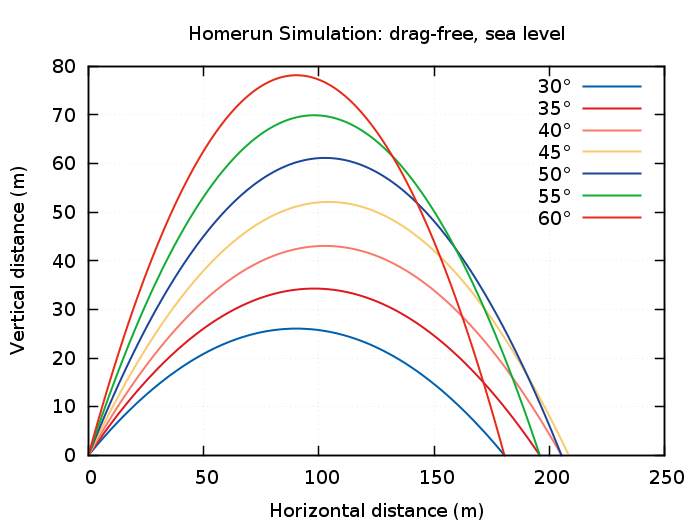
\includegraphics[width=3.75in]{drag0alt0.png}}
\caption{\it \small{Homerun trajectories for drag free case at sea level \label{fig1}}}
  \end{center}
\end{figure}

\begin{figure}[H]
  \begin{center}
\centerline{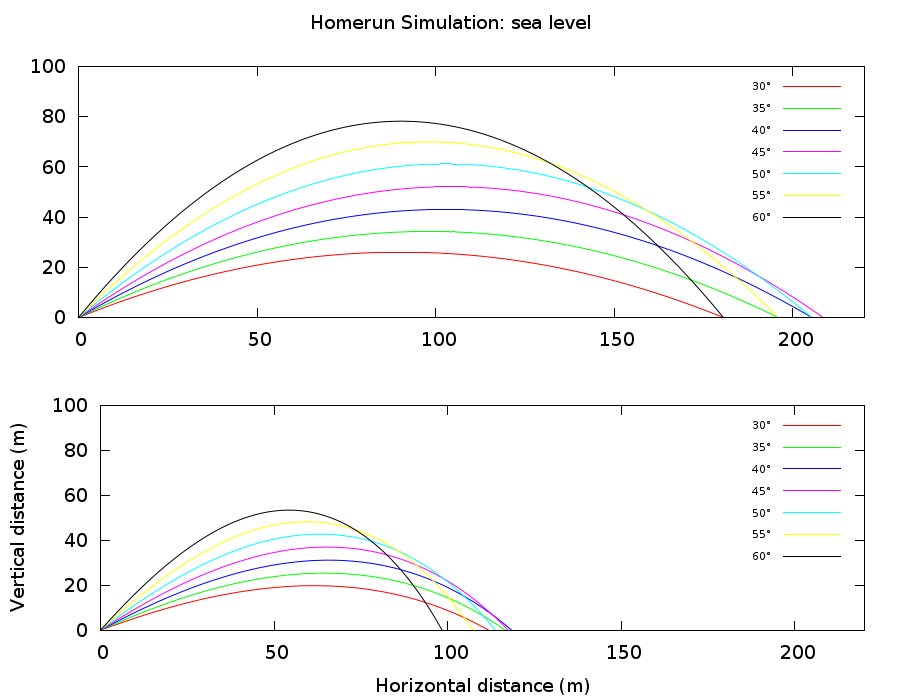
\includegraphics[width=3.25in]{fixkey2.png}}
\caption{\it \small{Homerun trajectories sea level \label{fig2}}}
  \end{center}
\end{figure}

\begin{figure}[H]
  \begin{center}
\centerline{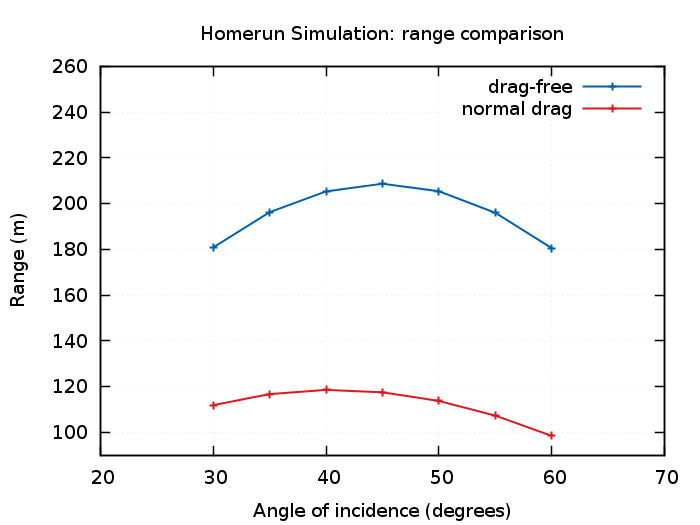
\includegraphics[width=3.25in]{rangevsangle.png}}
\caption{\it \small{Range comparison of drag-free and normal drag scenarios \label{fig3}}}
  \end{center}
\end{figure}
A baseball hit at sea level with an inital velocity of 45.2 m/s has a maximum range of 210 m, in the drag-free case.  This occurs 
when the ball is hit with an inital angle of 45 degrees.  
In the case of normal drag - such a baseball has a maximum range of 119 m, hit at an angle of 40 degrees.
\begin{figure}[H]
 \centerline{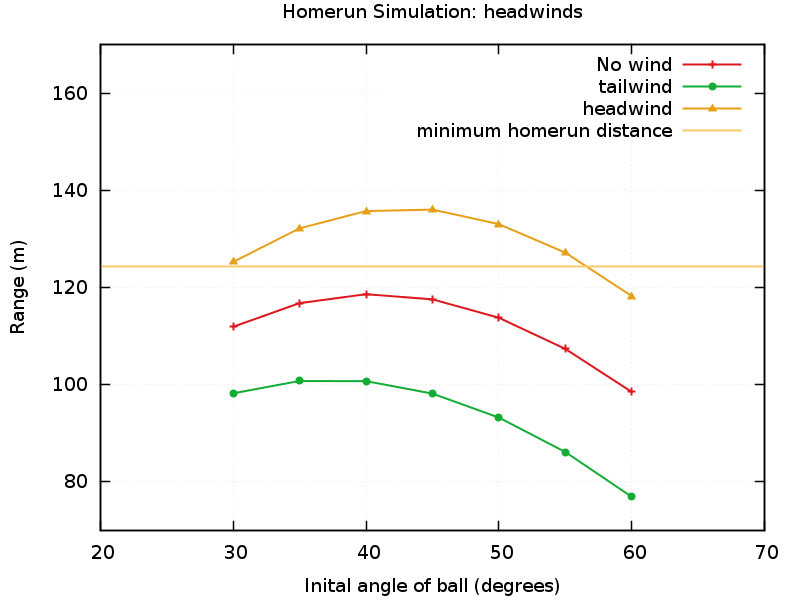
\includegraphics[width=2.9in]{rangeNY.png}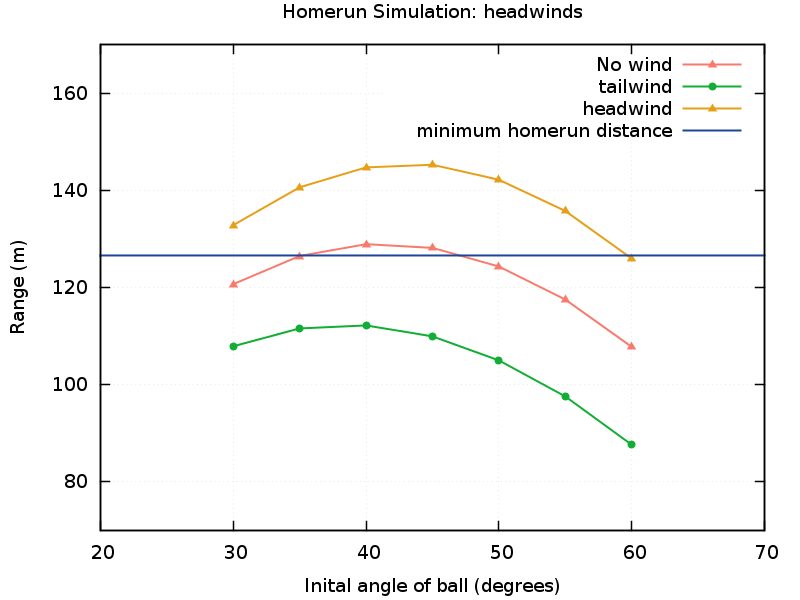
\includegraphics[width=2.9in]{rangedenver.png}}
\caption{\it \small{Range comparison with wind \label{fig4}}}
\end{figure}
A ball hit in New York must achieve a minimum distance of 124 meters in order to exceed the length of centerfield [3].  
In Denver a ball needs to travel 127 meters in order to be a centerfield homerun [4].  Other factors, such as rear wall height, 
are overlooked for simplicity.  In Denver (1600m) the drag is lower than in New York (0m) due to higher altitude causing lower 
air density and less drag.  A 15 mph tailwind increases a baseballs maximum range by 20 m.  A 15 mph headwind decreases a 
baseballs maximum range by 18 m.
\begin{figure}[H]
  \begin{center}
 \centerline{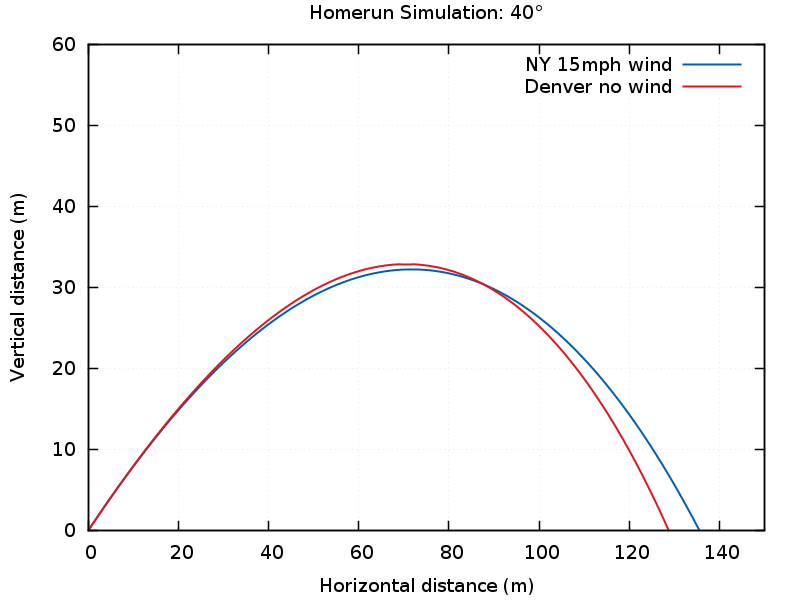
\includegraphics[width=2.9in]{finalplot2.png}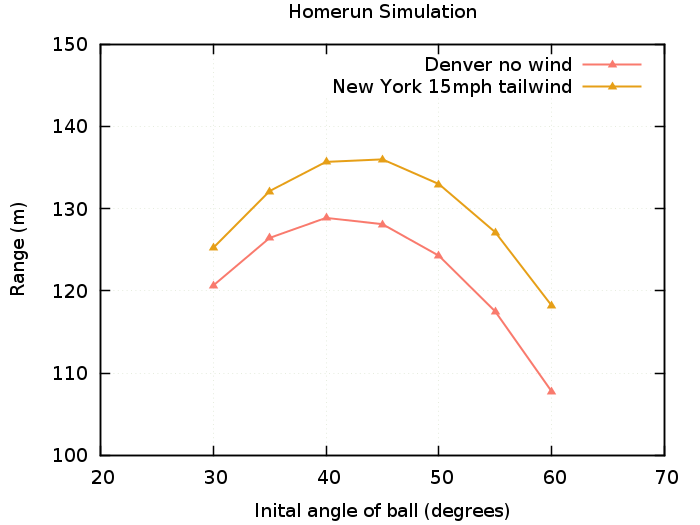
\includegraphics[width=2.9in]{finalplot.png}}
\caption{\it \small{Trajectory comparison of 40 degree scenarios on the left and maximum range comparison to~the~right \label{fig5}}}
  \end{center}
\end{figure}
In Denver, with normal drag and no wind, a baseball has a maximum range of 129 m.  In New York, with normal drag and a 
15 mph wind in the direction of the ball, a baseball has a maximum range of 136 m.  Wind in New York has more to do with range 
than Denvers'~altitude~does.



\section{Analysis}

Figure 1 shows the motion of a baseball struck with an inital velocity of 45.2 m/s at sea level, with no drag.  This figure shows 
that a ball will travel the furthest, in the x direction, when it is hit with an inital angle of 45 degrees.  Figure 2 shows the 
trajectories of homerun balls hit at sea level.  The higher plot is a simulation without drag while the lower plot shows normal 
drag trajectories.  Here it is shown that a ball hit with an inital angle of 40 dgerees will travel the furthest.  It is evident 
that drag decreases the range and lowers the angle needed to yiled the maximum range.



When there is a headwind the range of each angle is altered; as shown by figure 4.  
The graph on the left displays how the range in New York varies with different winds.  The graph to the right shows 
how the range in Denver in altered.  If the wind is in the same direction 
as the motion of the ball, a tailwind, the range increases.  If the wind is in the opposite direction as the ball, a headwind, 
the range decreases.  As shown in figure 4, no ball hit with mean velocity and no wind will reach far enough to be a homerun 
in centerfield of Yankee Stadium.  When the ball is assisted by wind this no longer holds true.  In Denver a ball at any angle 
between 30 and 60 degrees, with a mean strike velocity of 45.2 m/s and a 15 mph tailwind, 
will reach the 124.36 m minimum distance: resulting in a 
homerun [3].  This is a dramatic increase from the no wind case, where only balls hit with an inital angle over 30 and under 50 
degrees result in a homerun.  The maximum homerun range of a ball hit 
in Denver, with all other parameters being the same, exceeds the range of one hit in New York.



If a ball is hit in Denver with no wind, it will not go as far as a ball hit in New York with a 15 mph tailwind.  
This is depicted in figure 5.  From figure 5 we are able to see that with a 15 mph tailwind, a ball hit  
in New York will have a maximum range increased past that of a ball hit in Denver with no wind.  
Wind plays a larger role than altitude, in determining the range of a baseball.  
A signifcant enough increase in altitude will eventually overcome a range increase given by a tailwind.



\section{Conclusion}

A baseball hit in New York, under normal drag conditions, will not travel as far as one hit in Denver.  A drag force is one that 
opposes the motion of an object.  In the baseball simulation this was introduced as wind.  When the wind counters the motion 
of our ball its range decreases.  Only when aided by the wind can a ball hit in New York have a larger maximum range than 
one hit with no 
wind in Denver.  This shows that wind plays a larger role in determining homerun statistics than Denvers' altitude does.  By 
changing locations from New York to Denver the maximum range is increased from 119 m to  129 m, under normal drag conditions.  
Centerfield was used as the maximum distance a ball needs to travel in order to be considered a homerun.  
If readings we taken using either left or right field the range needed would be shorter and more home runs would be hit.



% the following \setlength is to force the bibliography to have no
% paragraph indentations.Can use vairous units--cm are used here.
\setlength{\parindent}{0cm}

\begin{thebibliography}{99}  % the trailing 99 controls some obscure format--just use

\bibitem{Landau} R. H. Landau and M. J. Paez, "Computational Physics, Problem Solving with Computers," (Wiley: New York) 1997.


\bibitem{Gorham} Gorham, Peter. "Physics 305 Differential Equations." P305lab7. Phys.hawaii.edu, 6 March 2015. Web. 12 Mar. 2015.


\bibitem{yankee} "Yankee Stadium." Yankee Stadium, New York Yankees Ballpark. Ballparks of Baseball, 2015. Web. 16 Mar. 2015.


\bibitem{coors} "Coors Field Information - Facts & Ground Rules." Colorado Rockies. MLB Advanced Media, 30 June 2014. Web. 16 Mar. 2015.


\end{thebibliography}

\section*{Appendix}
Various programs and plot files used in generating the graphs and data in this paper can be found online at: \\
\url{http://www2.hawaii.edu/~cmutnik/lab8.html}\\
All programs displayed here were written with the aid of Landau [1] and Gorham [2].



\end{document}

